\chapter{Introduction}
  \label{ch:intro}
  \begin{quotation}
    \small
    \textit{``It is now plain that about 75\% of the data we would like to have can be obtained from good ground-based sites''}

    -H. Johnson, 1966
  \end{quotation}

\section{All-sky Astronomy}


    All-sky astronomy is not new. Indeed, the notion of capturing a particular ``object'' or ``source'' with a camera and saving it for later investigation would be completely alien to the first astronomers and astronavigators. Absence of telescopes forced us to describe the sky in terms of its larger patterns, brightest characters. What is new however is the notion of preparing an archive of the sky itself for not only the research whims of a single investigator, team, institute, or even a single nation\- rather, all-sky surveys tend to be international endeavors in their production, and even more so in their utilization.

  %  \begin{table}
%      \caption{A timeline of all-sky surveys}
      %\label{tab:allsky-maps}
    %\end{table}

  \section{Infrared astronomy}

  Infrared astronomy was essentially non-existant as recently as the 1920s, if we judge by the first IR observations \citep{pettit22, pettit28}. Mainstream IR astronomy is perhaps much younger, only really taking off - literally- in the post-war era, via ballon and rocket borne experiments \citep{johnson66}. Compare this to visible wavelengths, a field so old we name it after the bio-evolutionary advent of sight, itself. Even radio astronomy with its own logistical and technological challenges, has been around since at least 1932.


  Despite the title quote above, astronomers were apprently not content to be constrained by atmospheric IR windows, even from the best of ground-based sites. Or perhaps interests have shifted so dramtically since 1966, that all of the investigations enabled by rocket-based, space-based, even Boeing 747-based IR astronomy would have bored 75\% of astronomers in the '60s. The meaning of ``far infrared'' has even redshifted, so to speak, from the \cite{johnson66} definition of ``4 to 22 um''.

   For our purposes, we consider the FIR to cover 60 to 550~$\mu$m, partially out of conveneince- FIR bands, in this paper, means the IRAS 60 and 100 micron, all four FIS bands, and the HFI~857~GHz and 545~GHz bands. The two IRC bands and the IRAS~12 and 25~$\mu$m bands we will refer to collectively as the MIR bands.

  The ability to map and archive the sky with satellites - not only in the optical and infrared, but well into the microwave regime - has enabled interdisciplinary research of the ISM. The merits of multiwavelength based investigations arise from the simple fact that the ISM is very complex- both in terms of the myriad forms of matter present - from plasmas to dust grains - and in countless physical processes at play.

   Consider the case of a dusty plasma, as in a supernova remnant or Hii region around an

   Studies of optical transients - a field accessible to amateur astronomers - can be validated by follow-ups in the infraredMulti-wavelength investigations not only allow us to examine the particular source we are interested in, but let us paint a full astrophysical picture. This is because the studying a given astrophysical phenomenon quickly requires us to control for confusing factors. Consider the case of thermal dust emission: attempting to trace the peak of thermal equilibirum dust emission, we will soon encounter deviations on the Wiens side- we know now that these mid to near IR deviations likely come from a smaller population of interstellar dust grains, with lower heat capacities \citep{purcell76, sellgren84,dwek86,draine01}.

  Astrochemists study of the molecular landscape of the ISM are

  Astrophysicists focused on the Milky Way itself are collaborating closely with those having more distant goals. \cite{johnson66} did not offer a definition of ``microwave'', though \cite{penzias65} had stumbled intro microwave astronomy a year before in their chance discovery of the cosmic microwave background (CMB). The CMB itself being relatively easy to model, on its own - latest measurements by Had the CMB been the only astronomical source of emission however, there would be no need for the following sections.

\section{Microwave foregrounds}

    The study of our galaxy itself via microwave emission is surely worth chapters of discussion. The reason that galactic microwave emission has gotten the amount of attention it has in recent years however has little to do with galactic astronomy. Rather, our galaxy presents an inconvenience to observational cosmology in that it 'contaminates' observations of the CMB. The avereage SED of the CMB is simple enough to model, with a 2.755~K blackbody function. This temperature however means that the peak occurs between several microwave foreground components, as displayed in Fig. \ref{fig:mw_foregrounds_demo_rOph}.

     temperature puts its emission peak right in the middle of severalThe difficult of decomposing the microwave sky into galactic ISM, extragalactic, and CMB components has brought the detailed decomposition of the microwave\-radio regime of ISM to the forefront of Planck Collaboration paper titles \citep{planckEarly11I,planck2013I,planck2015I}. This is true even though the CMB itself is relatively simple to model theoretically.
     - in the combined papers of the official numbered Planck Collaboration paper series, the word ``dust'' appears in 20; ``Galactic'' in 23; ``Galactic dust'' in 5. Without extragalactic research, there would be no need for the word ``foreground'' in describing galactic microwave emission.

    The ISM has intruded into cosmological studies perhaps most prominently with the first claimed detection of B-mode polarization \citep{hanson13, bicep214, flauger14} and the subsequent counter\-claim that this detection arose from galactic dust, and most recently the counter-counter suggestion that, after carefully accounting for galactic dust, the combined BICEP2/Planck detection of B-mode polarization appears validated \citep{planckIntL17}.\footnote{see \cite{sheehy17} for another take on Planck B-mode detection significance}. Similarly, More recently \cite{shimwell12} had noted a peculiar Sunyaev\-Zeldovich effect based galaxy cluster detection, AMI-CL~J0300+2613. \cite{perrott18} have since proposed that this may in fact arise from high galactic latitude dust via ``anomalous microwave emission'' (AME is described in the next section). In this way, enhanced wavelength coverage is both enabling and requiring deeper cross-disciplinary (galactic, extragalactic, CMB) collaboration.

  \subsection{Anomalous Microwave Emission}

      In our efforts to decompose and understand galactic microwave emission itself, there remains a constant antagonist. Anomalous microwave emission (AME) is a component of microwave emission in excess of 10 to 40~GHz predictions for known microwave emission mechansisms, lacking a confirmed physical mechanism. The term itself can be a bit confusing, as the word ``anomalous'' tends to imply an outlier lacking much evidence as to its cause, and with few emprical patterns. In this section we will explain that while there is indeed much mystery as to the exact mechanism(s) producing the AME, what causes its spectral variations, and what might be its physical carrier(s) - it is by now, perhaps less than anomalous. Following subsections will discuss the history of AME and the produced physical explanations, as well comparisons between the AME and infarred emission from interstellar dust.

    \begin{figure}
      \centering
      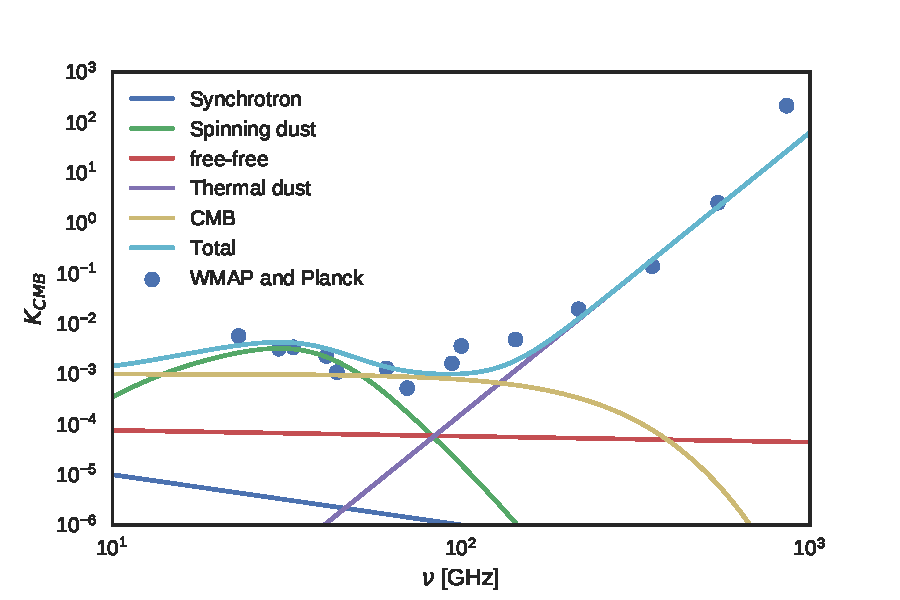
\includegraphics[width=\textwidth]{../Plots/ch_intro/mw_foregrounds_demo_rOph.pdf}
        \caption{An example of a potential makueup of microwave emission components. Photometry points are extracted from the Planck and WMAP all-sky maps, for a region well-known for prominant AME, $\rho$~Ophiuchus. \citep{planckxx11}}
      \label{fig:mw_foregrounds_demo_rOph}
    \end{figure}

    \begin{figure}
      \centering
      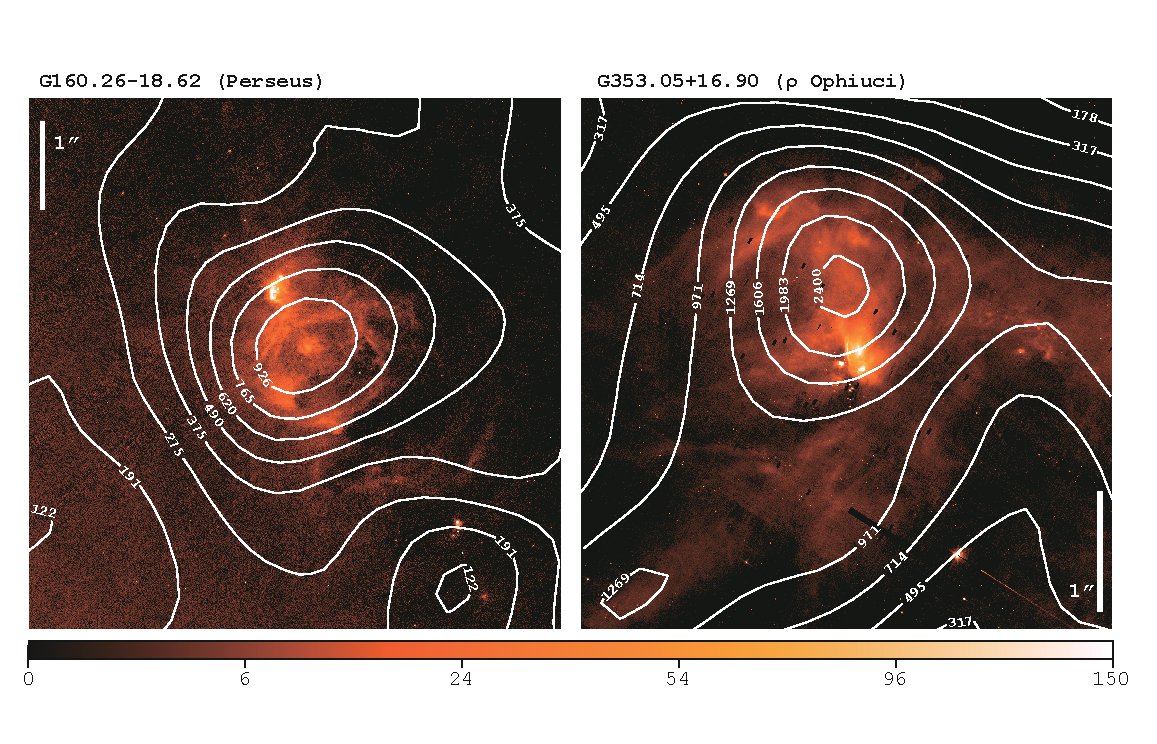
\includegraphics[width=\textwidth]{../Plots/ch_intro/AME_contours.pdf}
        \caption{Two AME prominent regions investigated by \cite{planckxx11, tibbs11}, $\rho$~Ophiuchus and Perseus, as they appear in the AKARI/IRC 9$\mu$m all-sky data at native resolution. White contours show AME at 1-degree resolution, extracted from the map by  \cite{planck15X}.}
      \label{fig:AME-contours}
    \end{figure}

    \subsubsection{Discovery and first explorations}

     Since its first detection in early microwave observations, AME has been found to be a widespread feature of the microwave Milky Way \citep{dickinson13r}. \cite{kogut96,deoliveiracosta97,leitch98} showed that the AME correlates very well with infrared emission from dust, via COBE/DIRBE and IRAS far-IR maps.

     From about 2002, the AME starts to become less of an anomaly, and more of an established -albeit mysterious- component of microwave emission. \cite{finkbeiner02} reported the first detection of a ``rising spectrum source at 8~−~10~GHz'' in a targeted observation, making the AME more than a statistical spectral outlier in CMB experiments. \cite{deoliveiracosta02} furher argued that this emission is in fact ``ubiquitous''. The exact mechanism and carrier/s remain mysterious however. Variations in the spectral profile of the AME signature,

     However there remains much mystery, except that the most likely source of the AME is interstellar dust. Several works have reported correlations between AME and thermal dust emission - but with some disagreement as to whether this correlation is improved in 12~$\mu$ emission vs. 100~$\mu$m emission \citep{ysard10a,tibbs11,hensley16}. Exactly which physical mechanisms are at play is still an open question, even if we assume a dusty AME origin. Even assuming a particular dust-based physical mechanism, we would still be puzzled as to the chemical composition and morphology of the carrier(s). We also lack an all-sky constraint on the emissivity of the AME spectrum at frequencies short of the WMAP cut-off, around 23~GHz.

  \subsubsection{Proposed explanations}

     From the observed spatial correlation between AME and dust emerged two prevailing hypotheses:

    1) Electric dipole emission by spinning small dust grains, a mechanism proposed in \cite{erickson57} and \cite{hoyle70}, with further discussion in \cite{ferrara94}. \cite{draine98b} give the earliest thorough description, with substantial updates contributed more recently by \cite{ysard10a}, \cite{ali-haimoud09}, \cite{hoang10} and several others. \cite{hensley17a} propose that such small spinning grains may consist primarily of silicates, and that this is allowed by observational upper-bounds of nanosilicate abudance, although nanosilicates have not yet been detected in the ISM. \cite{dickinson13r} provide a detailed overview of AME and spinning dust literature. An updated state of play of AME research has been submitted at the time of this writing (Dickinson, et al., submitted). Eq. \ref{eq:spinpower} gives the radiated power by spinning dust


        \begin{center}
        \begin{equation}
        P = {4\over9} {\mu^2\omega^4\over c^3}
        \label{eq:Pspin}
        \end{equation}
        \end{center

        \begin{equation}
        {\omega_T\over 2\pi} =
        \langle\nu^2\rangle^{1/2}
        \approx 5.60\times 10^9 a_{-7}^{-5/2}\xi^{-1/2}T_2^{1/2}~~~{\rm Hz}~,
        \label{eq:nurms}
        \end{equation}

    2) Magnetic dipole emission, caused by thermal fluctuations in grains with magnetic inclusions, proposed by \cite{draine99}.
     More recently, modeled spectra for potential candidate carriers have appeared in the literature: PAHs, grains with magnetic inclusions \citep{draine13, ali-haimoud14, hoang16a}.

    A third, but not widely accepted, possible explanation for AME is discussed in \cite{jones09}. They have suggested that the emissivity of dust, in the spectral range related to AME, could contain features caused by low temperature solid-state structural transitions.

    \subsubsection{Spinning dust}
     Spinning dust need not be the only emission mechanism, a convention as arisen in AME observational works. The photometric signature of the AME is frequently interepreted via spinning dust parameters \citep{ysard11,ali-haimoud10}. Archival all-sky AME data products exclusively assume a spinning dust SED templates.   \footnote{Both WMAP and Planck used a base template with 30~GHz peak frequency, and an assumed cold neutral medium evironment.} Using the ``spdust'' spinning dust SED model code to fit excess microwave foreground emission has become as commonplace as fitting a modified blackbody function to the far IR.

      We explore the case that the AME signature arises from spinning dust emission. If the AME is carried by spinning dust, the carrier should be small enough that it can be rotationally excited to frequencies in the range of 10-40~GHz, and must have a permanent electric dipole. Within contemporary dust SED models, only the polycyclic aromatic hydrocarbon family of molecules (PAHs), or nanoscale amorphous carbon dust fit these criteria. Those PAHs which have a permanent electric dipole (i.e. coranulene, but not symmetric molecules like coronene), can emit rotationally. However the carrier need not be carbon-based. Indeed, \cite{hensley17a} claim that AME can be explained without carbonaceous carriers, using only spinning nanosilicates.

     \subsubsection{Spinning PAHs?}
       Assuming the rotational emission model of \cite{draine98b}, the AME signature (consistent with peaked, continuum emission having a peak between 15 and 50~GHz ) implies very small oscillators (\textasciitilde{}10~nm).

       In any case, the PAH class of molecules are the only spinning dust candidate so far which show both: \\
       1) Evidence of abundance in the ISM at IR wavelengths, and \\
       2) A predicted range of dipole moments (on order of 1~debye), to produce the observed AME signature \citep{draine98b, lovas05, thorwirth07}. However, it should be noted that the current upper-bound on the abundance of nanosilicates, allows for a "spinning nanosilicate" explanation for the AME, as shown by \cite{hensley17a}. Due to the (apparently) continuous shape of the AME SED, a spinning dust explanation requires a distribution of dipole moments and/or rotational velocities of the carriers. Of course, the AME cannot simply be modeled by a distribution of carriers. Environmental factors affecting the rotational excitation of the carriers must be considered.

       \paragraph{A more testable hypothesis}
         At the time of this writing, there is no strong argument in the ltierature that either PAHs or nanosilicates are physically prefered by AME observations. The physical plausibility of rapidly spinning PAHs and of rapidly spinning nanosilicates to produce the AME have both been outlined. This plausibility however is contingent on the abundance of PAHs or nanosilicates with appropriate dipole moments, and in regions with suitable excitation environments.

         The arguments for or against particular carriers of the AME come from carrier abundance estimates and their statistical comparison with AME estiamtes. While neither nanosilicates nor any particular species of PAHs have been conclusively identified in the ISM, there is far more empiracal evidence for PAH-like dust there is for nanosilicates. Mid-infrared features associated with PAH-like aromatic materials have been observed. In fact, ``the PAH features'' are ubiquitous in the ISM \citep{giard94,onaka96,onaka00}, such that the carriers must be abundant.\footnote{ \cite{andrews15} strongly argue for the  existence of a dominant ``grandPAH'' class, containing 20 to 30 PAH species.} There has yet to be any detection of features related to nanosilicates. There is only an upper-bound from IRTS observations of \cite{onaka96} and calculations by \cite{li01}. \cite{hensley17a} argue that this upper-bound does not prohibit nanosilicates as the sole carriers of the AME.

     \subsection{Excitation factors}
       In the spinning dust model, there are several possible excitation factors for spinning dust. For the grains to have rotational velocities high enough to create the observed AME, they must be subject to strong excitation mechansisms. The dominant factors that would be giving grains their spin, are broken down by \cite{draine11} into basically two categories: 1) Collisional excitation. 2) Radiative excitation, the sum of which could lead to sufficient rotational velocities for sufficiently small grains. However the extent of excitation will depend on environmental conditions, i.e. there will be more frequent encounters with ions and atoms in denser regions (so long as the density is not high enough to coagulate the small grains), and more excitation due to photon emission with increasing ISRF strength \citep{ali-haimoud09, ali-haimoud14}. One of the strongest potential excitation mechansims listed in \cite{draine11} is that of negatively charged grains interacting with ions. Thus not only must we consider environmental factors, grain composition and size, but also the ionization state of the carriers. (For example, ionizaed vs. neutral PAHs.) The dependence of the observed AME on ISM density is modeled by \cite{ali-haimoud10}, demonstrating that denser regions may have a stronger AME component (although it can be observationally challenging to resolve dense vs. diffuse AME producing regions.)

       \subsection{AME vs. IR in the literature}
          The overall pattern among large-scale studies seems to show that all of the dust-tracing photometric bands correlate with the AME (and each other) to first-order.  On an all-sky, pixel-by-pixel basis, at 1$^{\circ}$ angular resolution, \cite{ysard10b} find that 12~$\mu$m emission, via IRAS, correlates slightly more strongly with AME (via WMAP) than with 100~$\mu$m emission.  They also find that scaling the IR intensity by the interstellar radiation field strength (given as $G_0$, a measure of ISRF relative to that of the solar neighborhood) improves both correlations. THey interpret this finding as evidence that AME is related to dust, and more closely related to the small stochastically emitting dust that is traced by 12~$\mu$m emission.

          However in a similar work, \cite{hensley16} report that the 12~$\mu$m emission (via WISE) correlates less tightly with AME than with thermal dust radiance, using the Planck Collaboration dust and AME component-separation maps \citep{planck15X}. Also at odds with \cite{ysard10b}, they report that AME correlates more strongly with 12~$\mu$m intensity than with the intensity scaled by the interstellar radiation field. They interpret this as AME and PAH emission both being correlated with the total dust radiance, but that there is no preferential relationship between PAHs and the AME.

         The story is no more clear when looking at the average properties of individual regions. \cite{planckXV} find that among 22 high-confidence ''AME regions" (galactic clouds such as the $\rho$~Ophiuchus cloud and the Perseus molecular cloud complex) AME vs. 12~$\mu$m  shows a marginally weaker correlation than AME vs. 100~$\mu$m (via IRAS). \cite{tibbs11} examined the AME-prominent Perseus Molecular Cloud complex, finding that while there is no clear evidence of a PAH-AME correlation, they do find a slight correlation between AME and  $G_0$.

          %       In this work, we attempt to reach some stronger consensus on the large-scale AME vs. IR-dust story, keeping in mind that resolution limitations are a could dilute more subtle connections between potential connections between dust IR emission and the anomalous foreground. In Ch. \hyperref[ch:datasources]{\ref*{ch:datasources}}, we describe the all-sky surveys and component maps used in this paper. The sources range from PAH-domianted MIR bands from AKARI and IRAS to FIR and microwave-derived maps from Planck Observatory. These bands are listed in Tab. \ref{tab:data} and are described in \ref{ch:datasources}. Our investigation is broken into two major approaches: a localized study of a particularly interesting AME region, around $\lambda$ Orionis, and an exploration into all-sky trends, to see if $\lambda$ Orionis results can be generalized. Chapter  \hyperref[ch:discussion]{\ref*{ch:discussion}} describes the conclusions of these 2 approaches, and compares them to previous AME vs. dust emission studies.

\section{Scope of this Dissertation}

  \subsection{An application of all-sky archival data}
    This is an astrophysical data archive based work. The primary goal is to highlight a particular application of multiwavelength (mid-IR to radio), cross-archive all-sky data analysis. We describe the interrelatedness between mid to far IR dust emission and possible microwave emission from dust. This is accomplished through an investigation of photometric all sky maps mainly from AKARI, IRAS, and Planck.

  \subsection{Testing the spinning PAH hypothesis}
    For the present work, we consider the spinning PAH hypothesis to have the highest degree of testability, due to the well-established presence of aromatic emisison feaetures in the ISM.  We do not argue against the physical plausibility of nanosilicates to produce the AME. Indeed, there is no argument to date that these potential physicalities are mutally exclusive, as long as both potential carriers are sufficiently abundant. Nor does spinning dust emission theoretically exclude magnetic dipole emission or microwave thermal dust emissivity fluctuations.

  \subsection{Limitations}
    We do not explore the modeling of microwave dust emission itself, rather the comparison of existing archival data and parameter maps. Modeling of the exact physical mechanism of the anomalous component of galactic microwave foreground emission from first principles is beyond the scope of this work. We consider this problem first on an all-sky basis, not focusing on any pre-selected object of the sky - in order to assess if there any general pattern between the IR and the AME, beyond the AME-dust correlation already described above. We then focus on a region highlighted by the Planck Collaboration as being especially worthy of further investigation \citep{planck15X}, and has a resolvable topology even at 1-degree resolution. Essentially all of the analyses and conclusions presented in this work apply to an angular scale of approximately 1-degree, and only for the given component separation methods (Solar system, galactic, extragalactic) used by each of the data providers.

  \subsection{Code availability}
    This dissertation is accompanied by a github repository\footnote{Available at: \url{https://github.com/aaroncnb/CosmicDust}.} Virtually all of the analyses code are available in that repository, in the form of Jupyter notebooks (along with the figures and the code used to generate them.) The dust SED fitting code is not part of that reposittory, but is described in Galliano et al. (in prep.)
